\section{Matrix Factorization Implementation}
To implement the matrix factorization mentioned in section 3.1, a smaller data set was chosen in order for us to carry out a comparison between the two approaches: the base method and the bias method (i.e., the method of matrix factorization that considers both user bias and item bias). 

\textbf{\textit{Dataset}}. The partial dataset is shown in Figure 4.9. The user-item rating matrix $\textit{R}$ is a $25 \times 100$ matrix, which represent 25 users and 100 items. Furthermore, we can see from the figure that  $\textit{R}$ is a sparse matrix (i.e. matrix with many zeros)
\begin{figure}
\centering
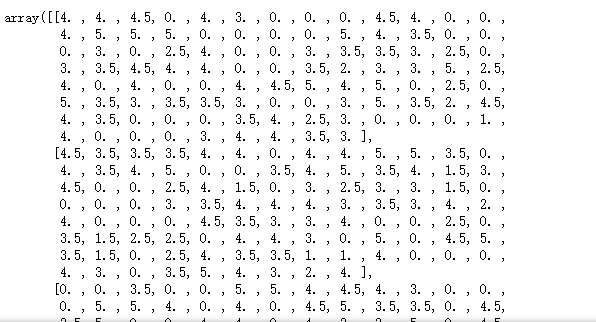
\includegraphics[scale =0.8]{figure/mf1.png}
\caption{Partial  of the user-item rating matrix \textit{R}}
\end{figure}

\textbf{\textit{Training}}.
Recall our loss function:
\begin{equation}
        \text { Loss }: J(p, q)=\min_{ q *, p * } \sum_{(u, i) \in K}\left(r_{u,i}-q_{i}^{T} p_{u}\right)^{2}+\lambda\left(\left\|q_{i}\right\|+\left\|p_{u}\right\|\right)^{2}
\end{equation}
Based on the methods proposed in \cite{mf1}, we use a stochastic gradient descent (SGD) algorithm to train two latent vector matrices: a user latent matrix \textit{p} and item latent matrix \textit{q}.By defining $e_{u,i}=r_{u,i}-q_{i}^{T} p_{u}$. We update the two matrices by the following formulas:
\begin{equation}
    q_{i} \leftarrow q_{i}+\eta\left(e_{u,i} p_{u}-\lambda q_{i}\right)
\end{equation}
\begin{equation}
    p_{u} \leftarrow p_{u}+\eta\left(e_{u,i} q_{i}-\lambda p_{u}\right)
\end{equation}
In the experiment, we set the number of latent features $k=2$, then we initiated the user matrix and item matrix with a size of $25 \times 2$ (i.e., number of users $\times$ number of latent features).
Furthermore, the learn rate$\eta=0.001$, regularization factor$\lambda = 0.1$ and iteration 1000 times.
\begin{figure}[htbp]
\centering
\subfigure[User latent matrix]{
\begin{minipage}[t]{0.5\linewidth}
\centering
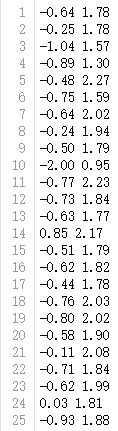
\includegraphics[scale=0.6]{figure/user1.png}
%\caption{fig1}
\end{minipage}%
}%
\subfigure[Item latent matrix (first 25 out of 100 items)]{
\begin{minipage}[t]{0.5\linewidth}
\centering
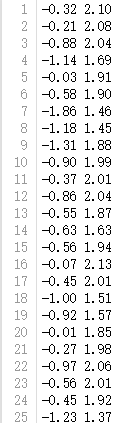
\includegraphics[scale=0.6]{figure/item1.png}
%\caption{fig2}
\end{minipage}%
}%
\centering
\caption{User and item matrix}
\end{figure} 
After iteration, we can get our user latent matrix \textit{p} and item latent matrix \textit{q}, as shown in figure 4.10. Then, by performing the inner product between these two latent matrices, we get the predicted user-item rating matrix $\hat{R}$, shown in Figure 4.11. Expressed by the formula: $\hat{R}$ = user latent matrix $\times$ item latent matrix$^\textbf{T}$.
\begin{figure}[htbp]
\centering
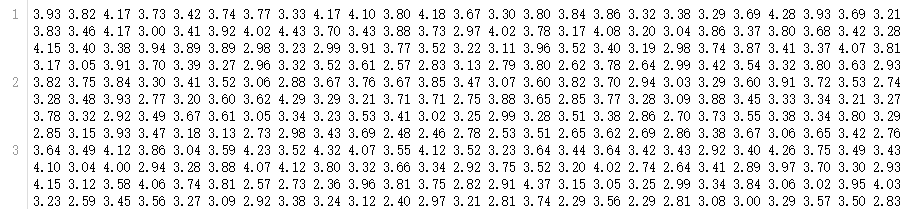
\includegraphics[scale =0.7]{figure/result1.png}
\caption{Predicated rating matrix $\hat{R}$ (Partial,first 3 out of 100 user's estimate rating)}
\end{figure}

\textbf{\textit{Adding bias}}.Now, we will experiment with the bias method, which considers both user bias and item bias. As mentioned before, when we consider the bias, then the loss function becomes:
\begin{equation}
    \operatorname{Loss}=\min _{q^{*}, p^{*}} \sum_{(u, i) \in K}\left(r_{u,i}-b_{u,i}-q_{i}^{T}p_{u}\right)^{2}+\lambda \left(\left\|q_{i}\right\|^{2}+\left\|p_{u}\right\|^{2}+b_{u}^{2}+b_{i}^{2}\right)
\end{equation}
The formula used to iterate over the user latent matrix and the item latent matrix becomes:
\begin{equation}
    q_{i} \leftarrow q_{i}+\eta\left(\left ( r_{u i}-q_{i}^{T} p_{u}-b_{u,i} \right ) p_{u}-\lambda q_{i}\right)
\end{equation}
\begin{equation}
    p_{u} \leftarrow p_{u}+\eta\left(\left ( r_{u i}-q_{i}^{T} p_{u}-b_{u,i} \right ) q_{i}-\lambda p_{u}\right)
\end{equation}
The rest of the steps are consistent with the base matrix factorization method.After the training, we get the user and item latent matrix based on the bias method. By the visualization method, Figure 4.12 plots the latent vectors of users and items in the two-dimensional coordinate. Through multiply the red dot coordinate by the blue cross’s coordinate in the figure, you can get the predicted rating score of user $u$ on item $i$.

\begin{figure}[htbp]
\centering
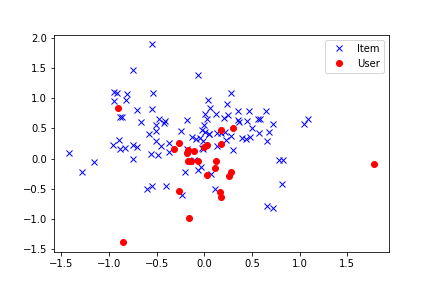
\includegraphics[scale =0.8]{figure/f6.png}
\caption{visualization of user and item latent vector}
\end{figure}

\textbf{\textit{Evaluation}}. To compare the performance between the base method and the bias method, Mean Square Error (MSE) is used to evaluate these two algorithms. In order not to lose generality, we conducted 10 experiments and took the average of the results. What is striking in Table 4.1 is the dramatic decline of MSE, when we consider user bias and item bias, the value of MSE is reduced by $20\%$ which proved that consider both user and item bias when
perform the matrix factorization is effective.


\begin{table}[htbp]
\centering
\begin{tabular}{lll}
\hline
            &\textbf{MSE}    & \textbf{Improvement rate} \\ \hline
Base method  $\hat{r}_{u,i}=q_{i}^{T}p_{u}$ & 0.6530 &                  \\
Bias method $\hat{\boldsymbol{r}}_{u,i}=b_{u,i}+q_{i}^{T} p_{u}$ & 0.5178 & 20.715\%        
\end{tabular}
\caption{Evaluation between base method and bias method}
\end{table}